\subsection{User view}
    \noindent \begin{minipage}{0.5\textwidth}
        \vspace{1cm}
        \fbox{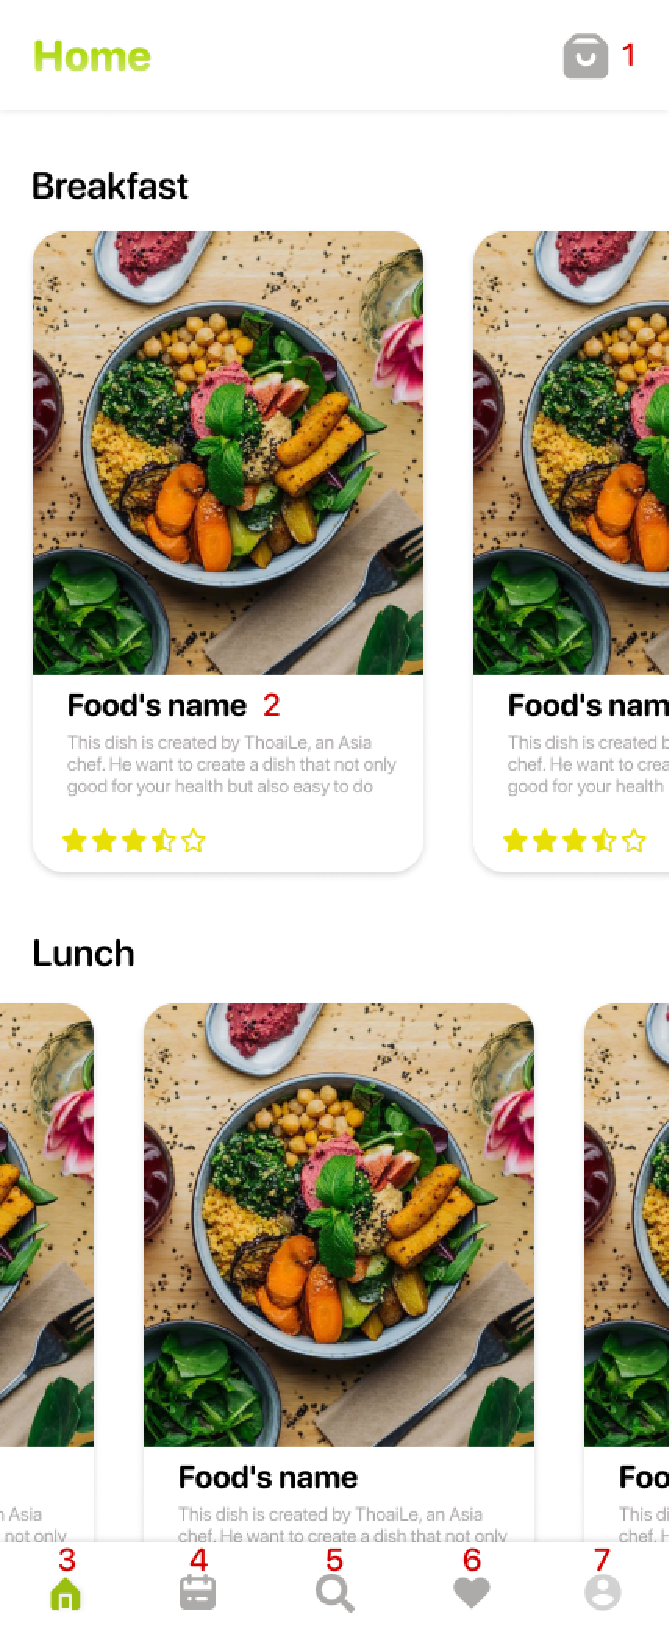
\includegraphics[width=\textwidth]{images/ui/Home.pdf}}
        \captionof{figure}{Trang chủ}
        \label{fig:nature}
    \end{minipage}
    \hspace{0.05\textwidth}
    \begin{minipage}{0.45\textwidth}
        \begin{tblr}{
            width=1\linewidth,
            hlines, 
            vlines,
            colspec={X[1]X[2]X[7]},
            columns = {valign = m, },
            column{1} = {halign = c},
            row{1} = {halign = c, valign = m, bg = lightgray, fg = black},
            }
            {\textbf{\#}} & \textbf{Type} & {\textbf{Mô tả}} \\
            1 & Button & Chuyển tới trang tạo lịch ăn\\
            2 & Link &  Chuyển tới trang chi tiết món ăn\\
            3 & Button & Chuyển đến trang Chủ\\
            4 & Button & Chuyển đến trang lịch ăn của tôi\\
            5 & Button & Chuyển đến trang tìm kiếm\\
            6 & Button & Chuyển đến trang món ăn ưa thích \\
            7 & Button & Chuyển đến trang thông tin cá nhân
        \end{tblr}
    \end{minipage}
    
    \noindent \begin{minipage}{0.5\textwidth}
        \vspace{1cm}
        \fbox{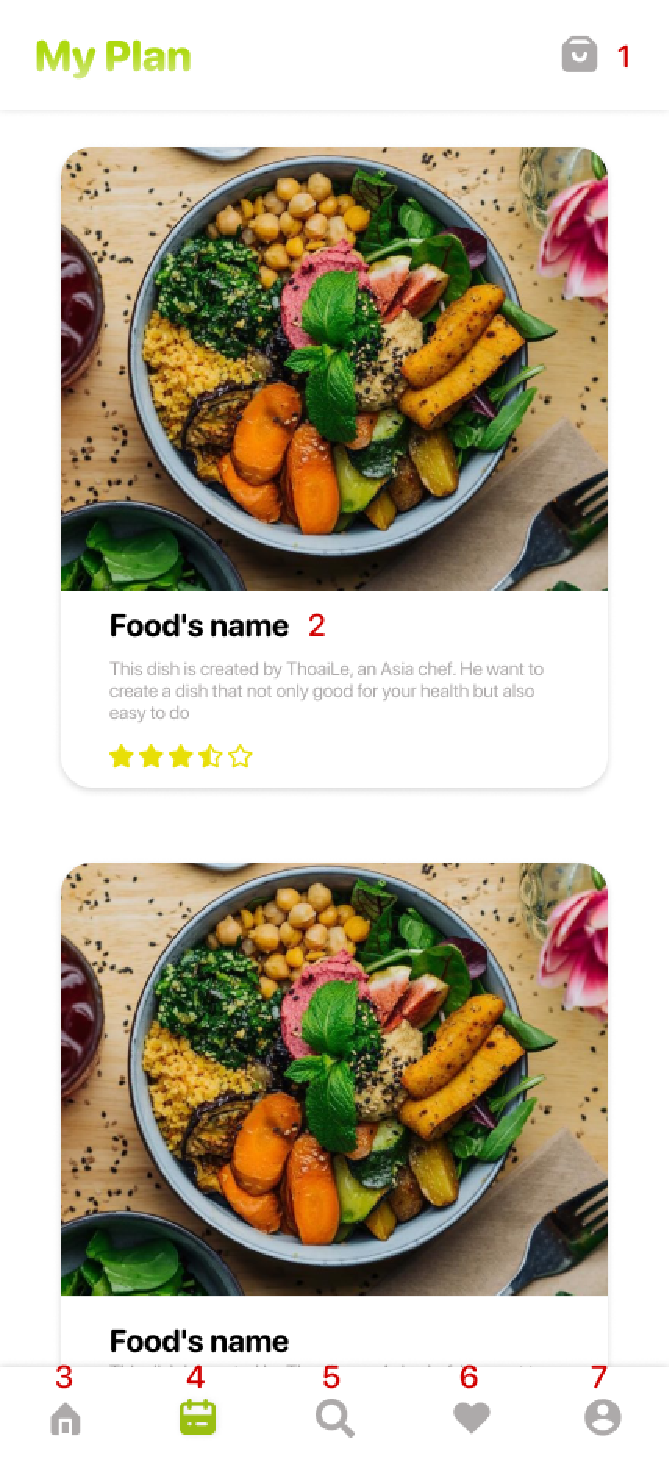
\includegraphics[width=\textwidth]{images/ui/My Plan.pdf}}
        \captionof{figure}{Trang lịch ăn của tôi}
        \label{fig:nature}
    \end{minipage}
    \hspace{0.05\textwidth}
    \begin{minipage}{0.45\textwidth}
        \begin{tblr}{
            width=1\linewidth,
            hlines, 
            vlines,
            colspec={X[1]X[2]X[7]},
            columns = {valign = m, },
            column{1} = {halign = c},
            row{1} = {halign = c, valign = m, bg = lightgray, fg = black},
            }
            {\textbf{\#}} & \textbf{Type} & {\textbf{Mô tả}} \\
            1 & Button & Chuyển tới trang tạo lịch ăn\\
            2 & Link &  Chuyển tới trang chi tiết món ăn\\
            3 & Button & Chuyển đến trang Chủ\\
            4 & Button & Chuyển đến trang lịch ăn của tôi\\
            5 & Button & Chuyển đến trang tìm kiếm\\
            6 & Button & Chuyển đến trang món ăn ưa thích \\
            7 & Button & Chuyển đến trang thông tin cá nhân \\
        \end{tblr}
    \end{minipage}
    
    \noindent \begin{minipage}{0.5\textwidth}
        \vspace{1cm}
        \fbox{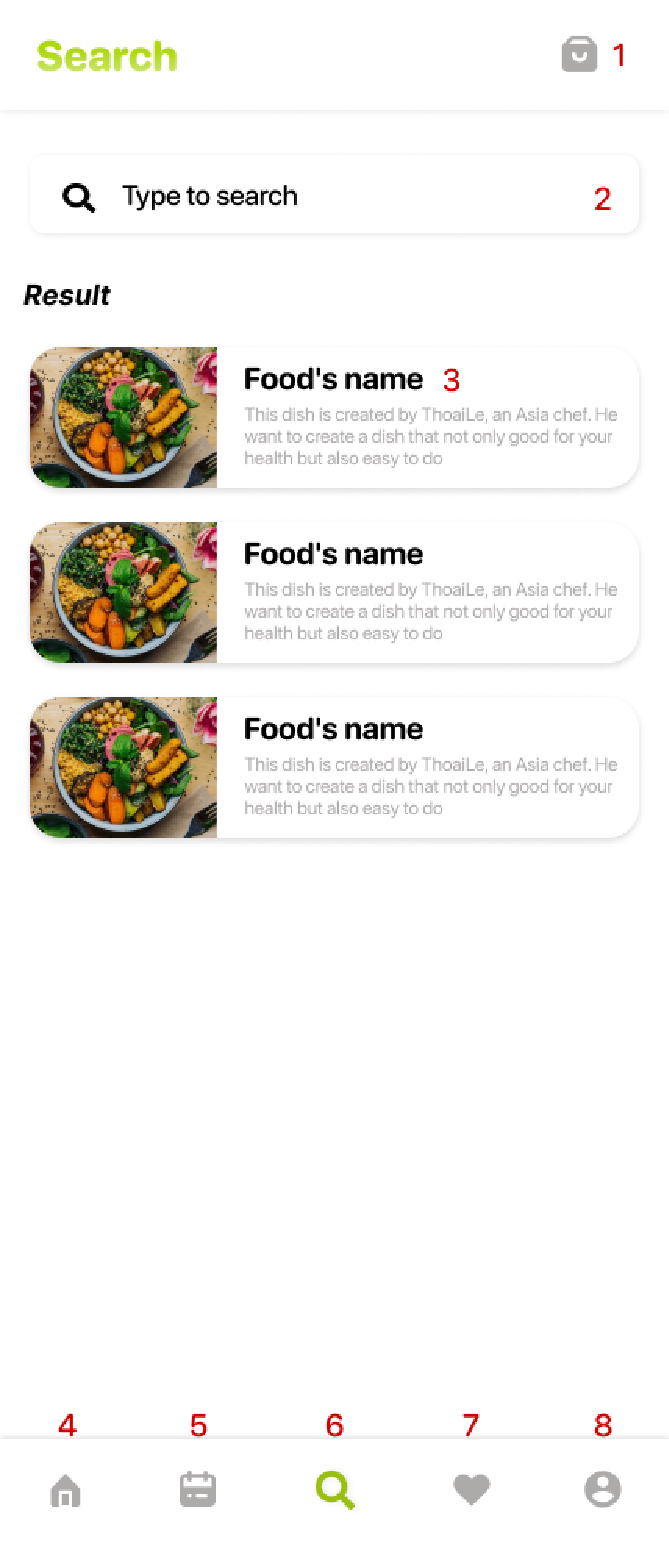
\includegraphics[width=\textwidth]{images/ui/Search.pdf}}
        \captionof{figure}{Trang tìm kiếm}
        \label{fig:nature}
    \end{minipage}
    \hspace{0.05\textwidth}
    \begin{minipage}{0.45\textwidth}
        \begin{tblr}{
            width=1\linewidth,
            hlines, 
            vlines,
            colspec={X[1]X[2]X[7]},
            columns = {valign = m, },
            column{1} = {halign = c},
            row{1} = {halign = c, valign = m, bg = lightgray, fg = black},
            }
            {\textbf{\#}} & \textbf{Type} & {\textbf{Mô tả}} \\
            1 & Button & Chuyển tới trang tạo lịch ăn\\
            2 & Input &  Người dùng nhập món ăn cần tìm\\
            3 & Link &  Chuyển tới trang chi tiết món ăn\\
            4 & Button & Chuyển đến trang Chủ\\
            5 & Button & Chuyển đến trang lịch ăn của tôi\\
            6 & Button & Chuyển đến trang tìm kiếm\\
            7 & Button & Chuyển đến trang món ăn ưa thích \\
            8 & Button & Chuyển đến trang thông tin cá nhân \\
        \end{tblr}
    \end{minipage}
    
    \noindent \begin{minipage}{0.5\textwidth}
        \vspace{1cm}
        \fbox{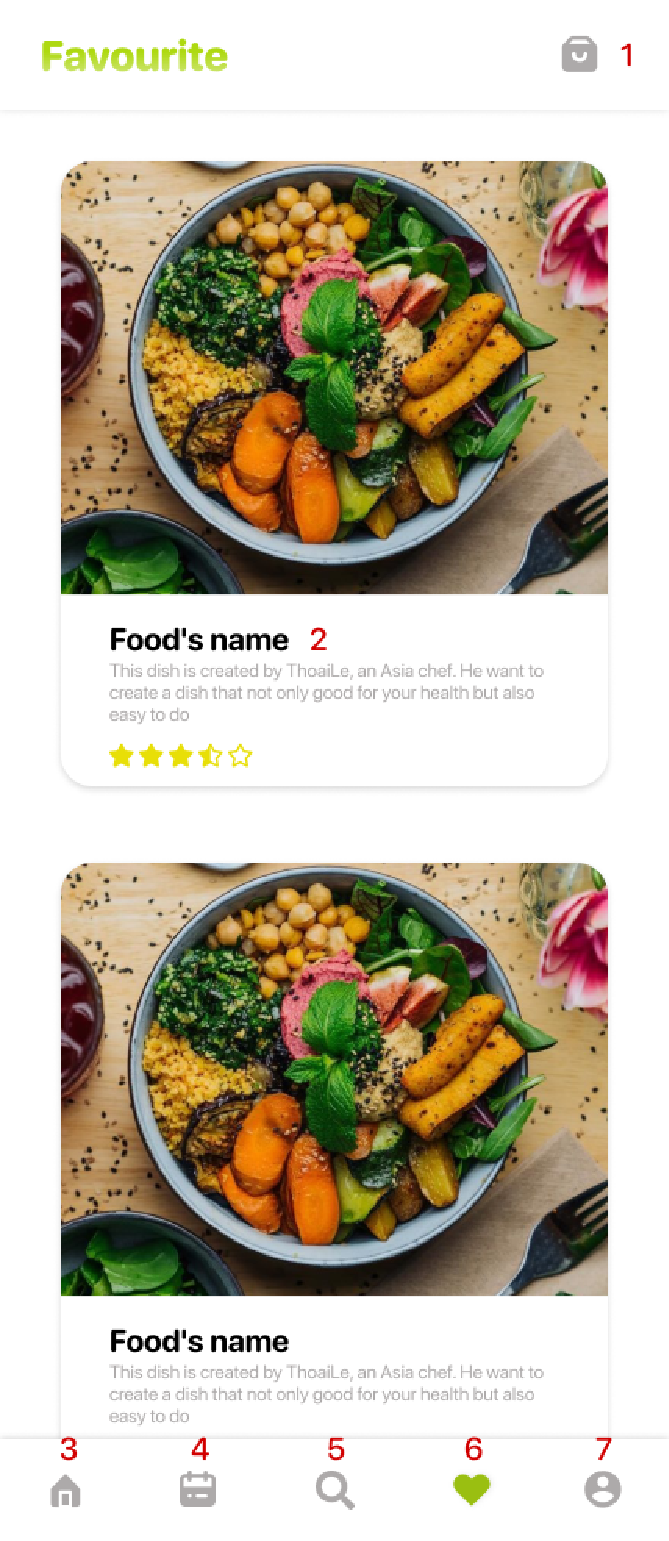
\includegraphics[width=\textwidth]{images/ui/Favorite.pdf}}
        \captionof{figure}{Trang món ăn ưa thích}
        \label{fig:nature}
    \end{minipage}
    \hspace{0.05\textwidth}
    \begin{minipage}{0.45\textwidth}
        \begin{tblr}{
            width=1\linewidth,
            hlines, 
            vlines,
            colspec={X[1]X[2]X[7]},
            columns = {valign = m, },
            column{1} = {halign = c},
            row{1} = {halign = c, valign = m, bg = lightgray, fg = black},
            }
            {\textbf{\#}} & \textbf{Type} & {\textbf{Mô tả}} \\
            1 & Button & Chuyển tới trang tạo lịch ăn\\
            2 & Link &  Chuyển tới trang chi tiết món ăn\\
            3 & Button & Chuyển đến trang Chủ\\
            4 & Button & Chuyển đến trang lịch ăn của tôi\\
            5 & Button & Chuyển đến trang tìm kiếm\\
            6 & Button & Chuyển đến trang món ăn ưa thích \\
            7 & Button & Chuyển đến trang thông tin cá nhân \\
        \end{tblr}
    \end{minipage}
    
    \noindent \begin{minipage}{0.5\textwidth}
        \vspace{1cm}
        \fbox{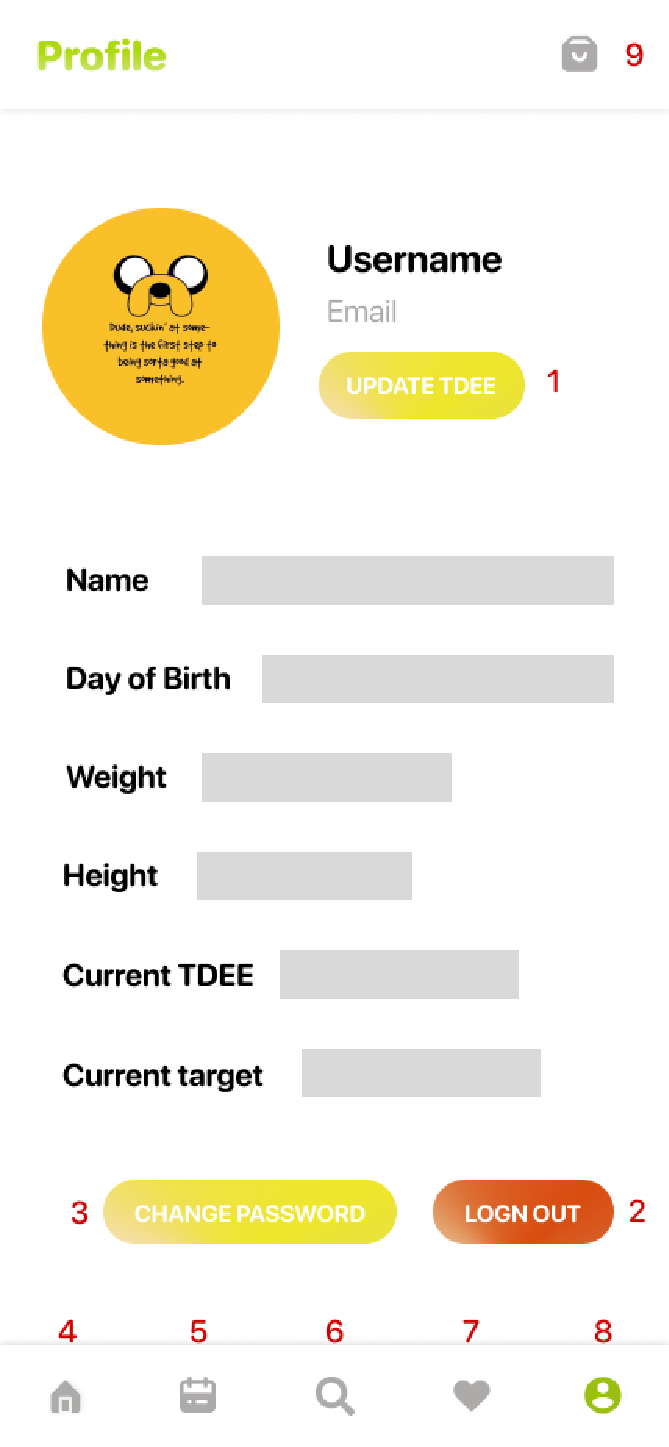
\includegraphics[width=\textwidth]{images/ui/Profile - user.pdf}}
        \captionof{figure}{Trang thông tin cá nhân}
        \label{fig:nature}
    \end{minipage}
    \hspace{0.05\textwidth}
    \begin{minipage}{0.45\textwidth}
        \begin{tblr}{
            width=1\linewidth,
            hlines, 
            vlines,
            colspec={X[1]X[2]X[7]},
            columns = {valign = m, },
            column{1} = {halign = c},
            row{1} = {halign = c, valign = m, bg = lightgray, fg = black},
            }
            {\textbf{\#}} & \textbf{Type} & {\textbf{Mô tả}} \\
            1 & Button & Chuyển tới tính toán TDEE\\
            2 & Button &  Đăng xuất và trở về trang đăng nhập\\
            3 & Button & Chuyển đến trang thay đổi mật khẩu\\
            4 & Button & Chuyển đến trang Chủ\\
            5 & Button & Chuyển đến trang lịch ăn của tôi\\
            6 & Button & Chuyển đến trang tìm kiếm\\
            7 & Button & Chuyển đến trang món ăn ưa thích \\
            8 & Button & Chuyển đến trang thông tin cá nhân \\
            9 & Button & Chuyển đến trang tạo lịch ăn \\
        \end{tblr}
    \end{minipage}
    
    \noindent \begin{minipage}{0.5\textwidth}
        \vspace{1cm}
        \fbox{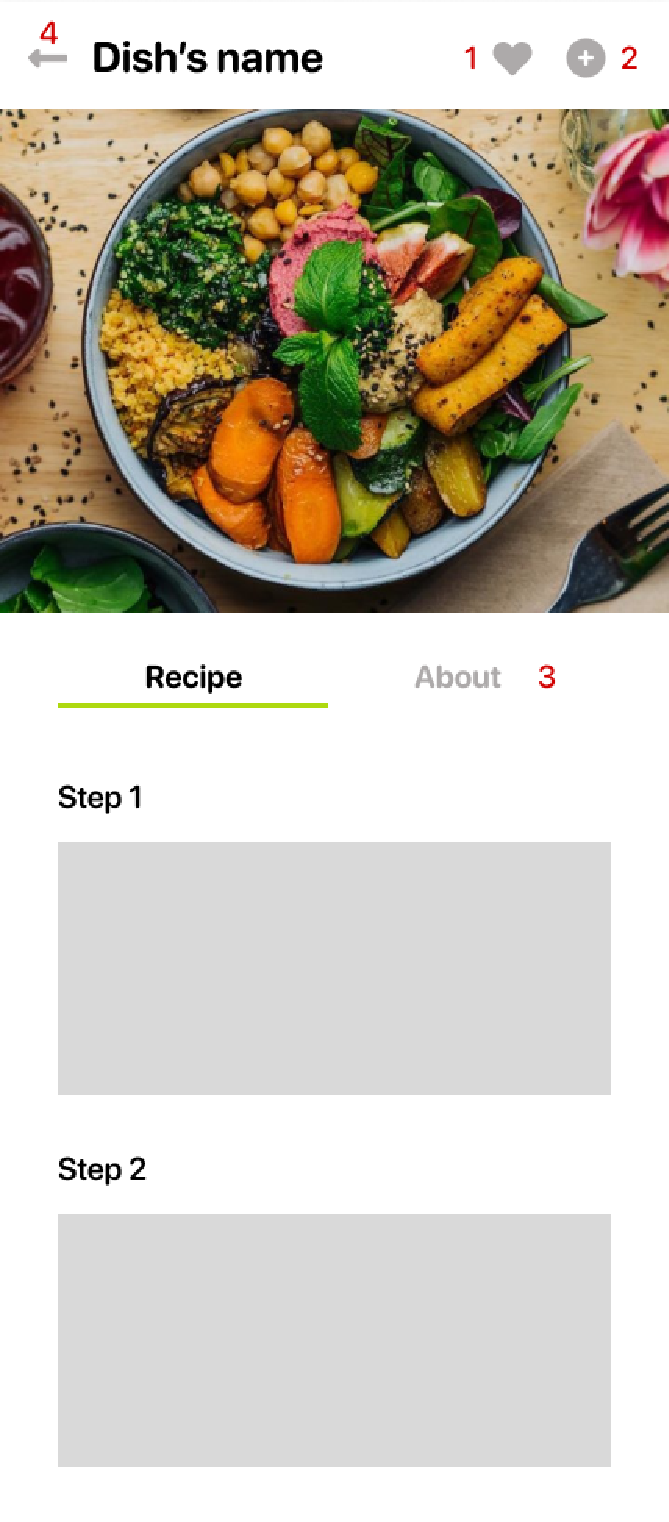
\includegraphics[width=\textwidth]{images/ui/Dish detail - recipe.pdf}}
        \captionof{figure}{Trang chi tiết món ăn (công thức)}
        \label{fig:nature}
    \end{minipage}
    \hspace{0.05\textwidth}
    \begin{minipage}{0.45\textwidth}
        \begin{tblr}{
            width=1\linewidth,
            hlines, 
            vlines,
            colspec={X[1]X[2]X[7]},
            columns = {valign = m, },
            column{1} = {halign = c},
            row{1} = {halign = c, valign = m, bg = lightgray, fg = black},
            }
            {\textbf{\#}} & \textbf{Type} & {\textbf{Mô tả}} \\
            1 & Button & Món ăn sẽ được thêm vào danh sách ưa thích\\
            2 & Button &  Thêm món ăn vào danh sách tạo lịch ăn\\
            3 & Button & Chuyển sang tab thông tin\\
            4 & Button & Quay trở lại trang trước đó \\
        \end{tblr}
    \end{minipage}
    
    \noindent \begin{minipage}{0.5\textwidth}
        \vspace{1cm}
        \fbox{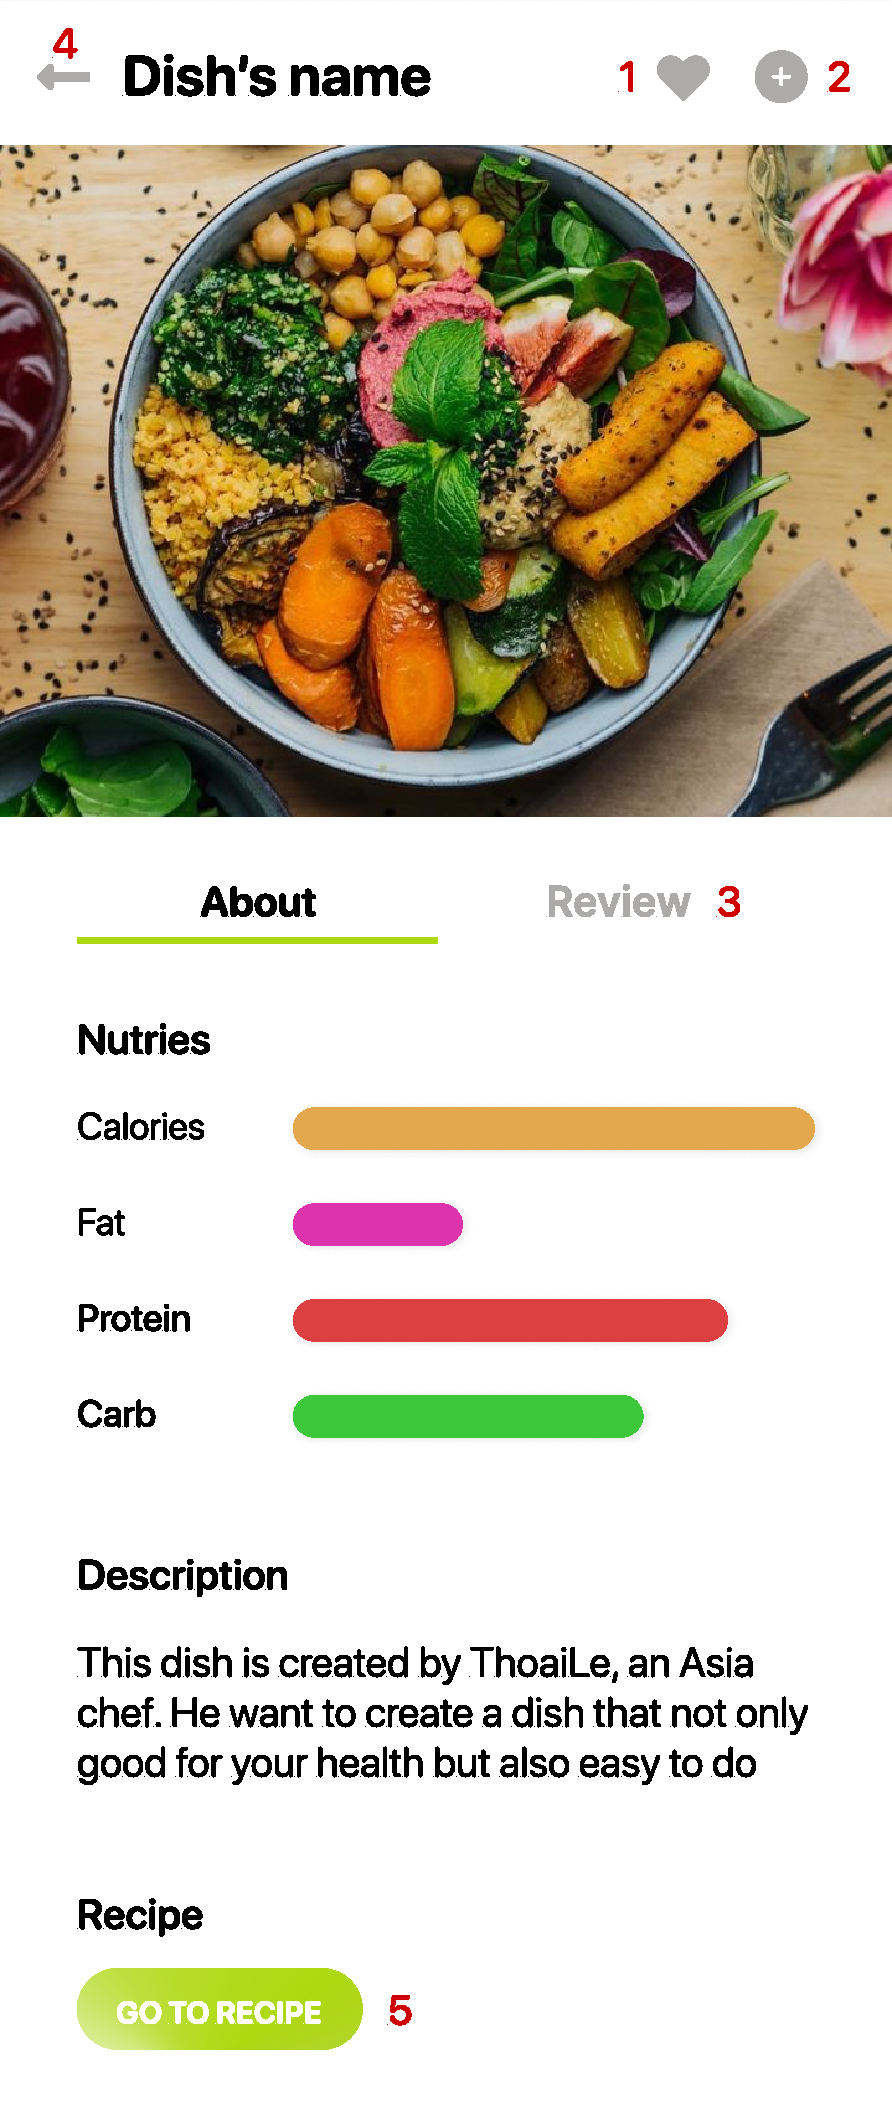
\includegraphics[width=\textwidth]{images/ui/Dish detail - about.pdf}}
        \captionof{figure}{Trang chi tiết món ăn (Thông tin)}
        \label{fig:nature}
    \end{minipage}
    \hspace{0.05\textwidth}
    \begin{minipage}{0.45\textwidth}
        \begin{tblr}{
            width=1\linewidth,
            hlines, 
            vlines,
            colspec={X[1]X[2]X[7]},
            columns = {valign = m, },
            column{1} = {halign = c},
            row{1} = {halign = c, valign = m, bg = lightgray, fg = black},
            }
            {\textbf{\#}} & \textbf{Type} & {\textbf{Mô tả}} \\
            1 & Button & Món ăn sẽ được thêm vào danh sách ưa thích\\
            2 & Button &  Thêm món ăn vào danh sách tạo lịch ăn\\
            3 & Button & Chuyển sang tab công thức\\
            4 & Button & Đánh giá món ăn \\
            5 & Input & Thêm bình luận cho món ăn \\
            6 & Button & Xác nhận đánh giá món ăn \\
            7 & Button & Quay lại trang trước đó \\
        \end{tblr}
    \end{minipage}
    
    \noindent \begin{minipage}{0.5\textwidth}
        \vspace{1cm}
        \fbox{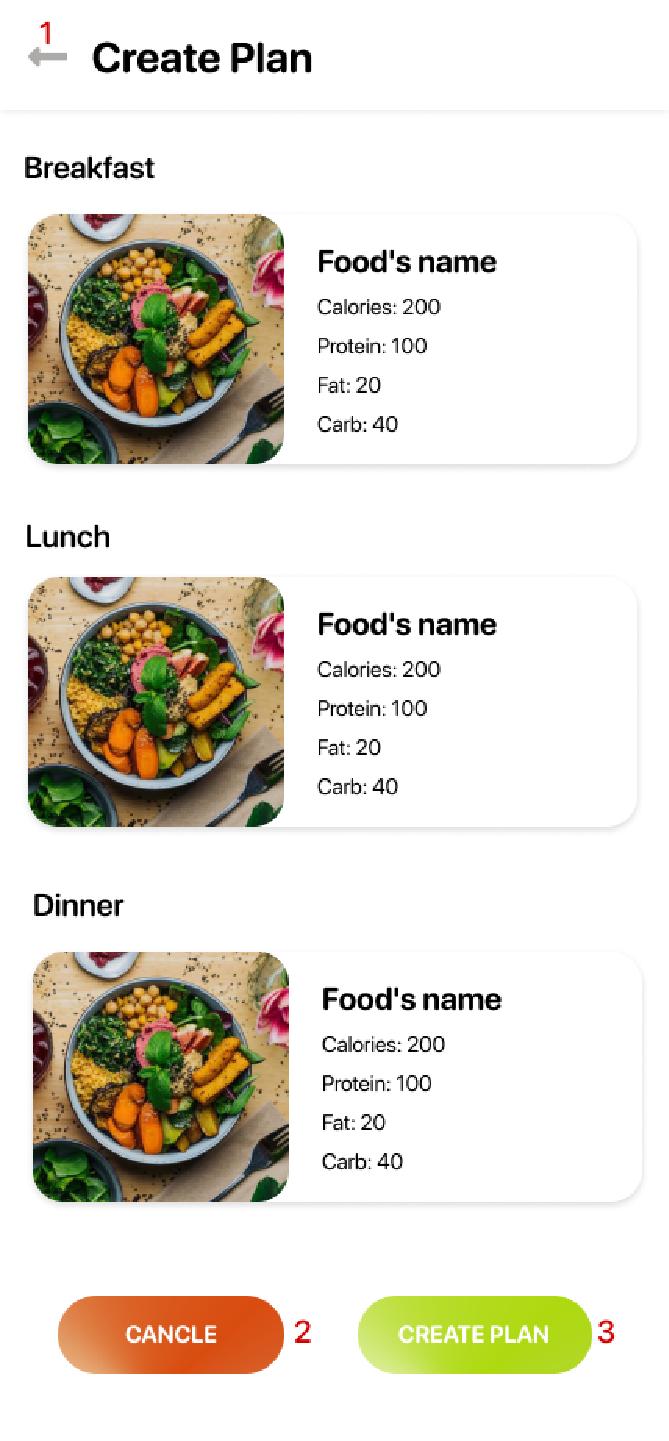
\includegraphics[width=\textwidth]{images/ui/Create plan.pdf}}
        \captionof{figure}{Trang tạo lịch ăn}
        \label{fig:nature}
    \end{minipage}
    \hspace{0.05\textwidth}
    \begin{minipage}{0.45\textwidth}
        \begin{tblr}{
            width=1\linewidth,
            hlines, 
            vlines,
            colspec={X[1]X[2]X[7]},
            columns = {valign = m, },
            column{1} = {halign = c},
            row{1} = {halign = c, valign = m, bg = lightgray, fg = black},
            }
            {\textbf{\#}} & \textbf{Type} & {\textbf{Mô tả}} \\
            1 & Button & Quay lại trang trước đó \\
            2 & Button & Hủy tạo lịch ăn, quay lại trang trước đó \\
            3 & Button & Xác nhận tạo lịch ăn, các món ăn sẽ được hiện ở trang lịch ăn của tôi \\
        \end{tblr}
    \end{minipage}
    
    \noindent \begin{minipage}{0.5\textwidth}
        \vspace{1cm}
        \fbox{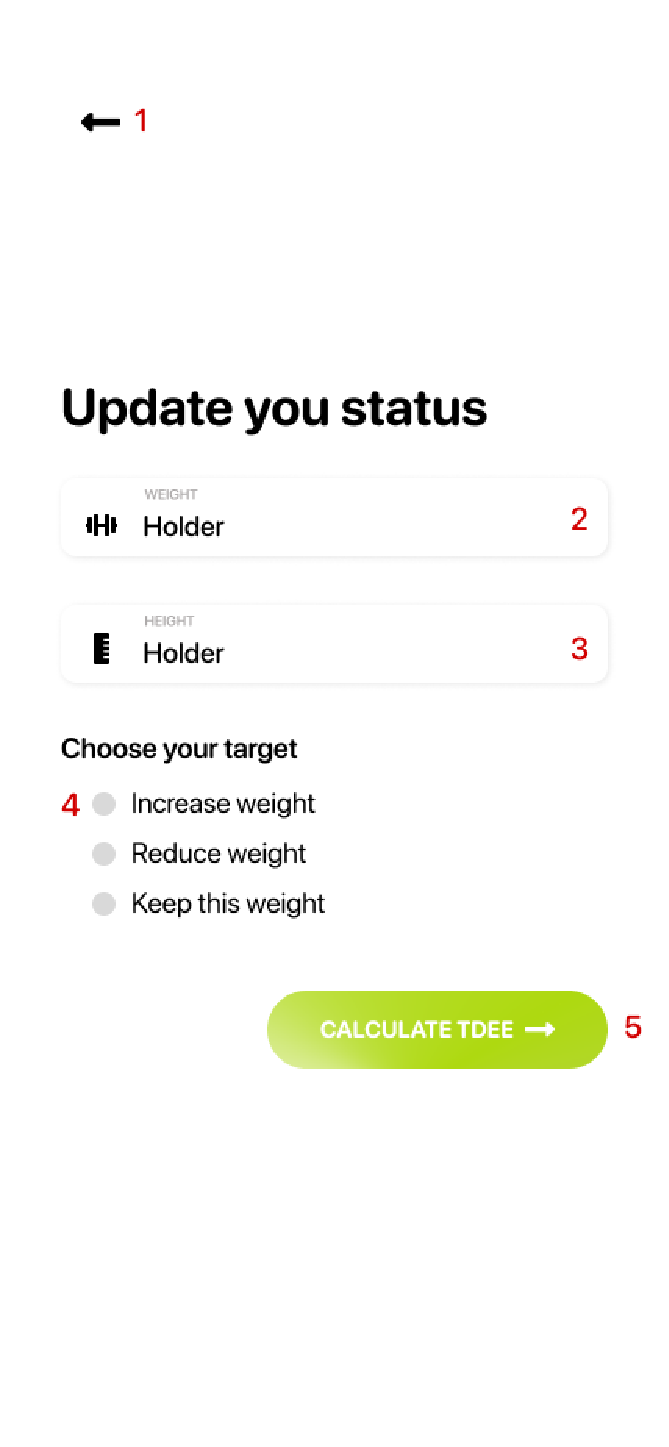
\includegraphics[width=\textwidth]{images/ui/Calculate TDEE.pdf}}
        \captionof{figure}{Trang tính TDEE}
        \label{fig:nature}
    \end{minipage}
    \hspace{0.05\textwidth}
    \begin{minipage}{0.45\textwidth}
        \begin{tblr}{
            width=1\linewidth,
            hlines, 
            vlines,
            colspec={X[1]X[2]X[7]},
            columns = {valign = m, },
            column{1} = {halign = c},
            row{1} = {halign = c, valign = m, bg = lightgray, fg = black},
            }
            {\textbf{\#}} & \textbf{Type} & {\textbf{Mô tả}} \\
            1 & Button & Quay lại trang trước đó \\
            2 & Input & Nhập thông tin cân nặng \\
            3 & Input & Nhập thông tin chiều cao \\
            4 & Choose button & Chọn mục tiêu \\
            5 & Button & Xác nhận thông tin, tính toán TDEE \\
        \end{tblr}
    \end{minipage}
